\documentclass[tikz,border=8pt]{standalone}
\usetikzlibrary{arrows.meta}
\begin{document}
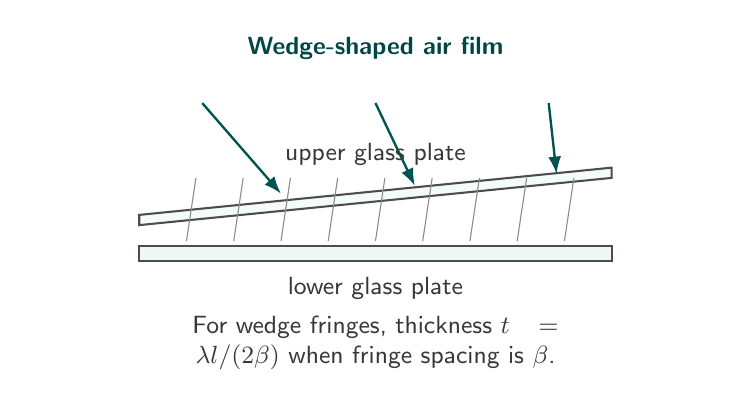
\begin{tikzpicture}[
  line/.style={draw=black!70,line width=0.75pt},
  ray/.style={-{Latex[length=2.2mm]},draw=teal!65!black,line width=0.85pt},
  label/.style={font=\sffamily\small,text=black!78},
  title/.style={font=\sffamily\bfseries\small,text=teal!55!black},
]
\node[title] at (0,2.7) {Wedge-shaped air film};
\draw[line,fill=teal!6] (-3,0) rectangle (3,0.18);
\draw[line,fill=teal!4] (-3,0.45)--(3,1.05)--(3,1.18)--(-3,0.58)--cycle;
\draw[ray] (-2.2,2.0)--(-1.2,0.85);
\draw[ray] (0,2.0)--(0.5,0.95);
\draw[ray] (2.2,2.0)--(2.3,1.1);
\node[label] at (0,-0.35) {lower glass plate};
\node[label] at (0,1.35) {upper glass plate};
\foreach \x in {-2.4,-1.8,...,2.4}{\draw[black!45] (\x,0.25)--(\x+0.12,1.05);}
\node[label,align=center,text width=8.6cm] at (0,-1.05)
  {For wedge fringes, thickness $t=\lambda l/(2\beta)$ when fringe spacing is $\beta$.};
\end{tikzpicture}
\end{document}
